% Standalone render of generated_intraday_dh/table_rule_by_strategy_dh_holdclose_1200.tex
% Build: pdflatex -interaction=nonstopmode rule_by_strategy_dh_holdclose_1200.tex
\documentclass{article}
\usepackage[landscape,margin=0.5in]{geometry}
\usepackage{booktabs}
\usepackage{amsmath}
\usepackage{graphicx}
\pagestyle{empty}

\begin{document}
\begin{center}
\textbf{0DTE nearest-OTM straddle: per-rule return summary, entry 12:00 ET, held to cash-settle, models compared on the same 866 days}\\[1.5ex]
% AUTO-GENERATED by writeup/make_rule_by_strategy_intraday_tex.py -- do not edit.
% Source: results/atm_straddle_intraday/rule_by_strategy/1200/rule_by_strategy_*.csv
\begingroup\small\setlength{\tabcolsep}{3.6pt}
\begin{tabular}{lrrrrrrrrrrrr}
\toprule
& $n$ & mean & std & min & max & skew & ex.\ kurt & $t$ & Sharpe$_{\mathrm{clk}}$ & $n_{\mathrm{buy}}$ & \%buy & Sharpe$^{\times}_{\mathrm{clk}}$ \\
\midrule
\multicolumn{13}{l}{\emph{Short volatility (always short)}} \\
all models (no forecast) & 866 & 0.087 & 0.434 & -2.97 & 0.93 & -1.48 & 5.45 & 5.88 & 3.17 & 0 & 0.0 & 2.58 \\
\midrule
\multicolumn{13}{l}{\emph{$\mathrm{sign}(s)$ ($\pm 1$ on the sign of $s$)}} \\
baseline (HAR + calendar OLS) & 866 & 0.025 & 0.442 & -2.97 & 1.98 & -0.67 & 4.12 & 1.68 & 0.91 & 364 & 42.0 & 0.33 \\
block-diagonal ridge & 866 & 0.033 & 0.442 & -2.06 & 2.97 & 0.26 & 3.91 & 2.22 & 1.20 & 367 & 42.4 & 0.62 \\
block-diagonal ridge, without the FOMC columns & 866 & 0.030 & 0.442 & -2.06 & 2.97 & 0.27 & 3.90 & 2.03 & 1.09 & 379 & 43.8 & 0.51 \\
LightGBM$^{\dagger}$ & 866 & 0.040 & 0.441 & -2.10 & 2.97 & 0.09 & 3.97 & 2.67 & 1.44 & 360 & 41.6 & 0.86 \\
XGBoost$^{\dagger}$ & 866 & 0.023 & 0.442 & -2.06 & 2.97 & 0.07 & 3.95 & 1.52 & 0.82 & 372 & 43.0 & 0.24 \\
lasso (causally tuned)$^{\dagger}$ & 866 & 0.025 & 0.442 & -2.97 & 1.98 & -0.60 & 4.10 & 1.64 & 0.88 & 385 & 44.5 & 0.30 \\
lasso ($\alpha=10^{-4}$) & 866 & 0.036 & 0.441 & -2.06 & 2.97 & 0.22 & 3.92 & 2.39 & 1.29 & 372 & 43.0 & 0.71 \\
elastic net (causally tuned)$^{\dagger}$ & 866 & 0.025 & 0.442 & -2.10 & 2.97 & 0.08 & 3.95 & 1.67 & 0.90 & 382 & 44.1 & 0.32 \\
\bottomrule
\end{tabular}
\endgroup

\end{center}
\vspace{1ex}
\begin{center}
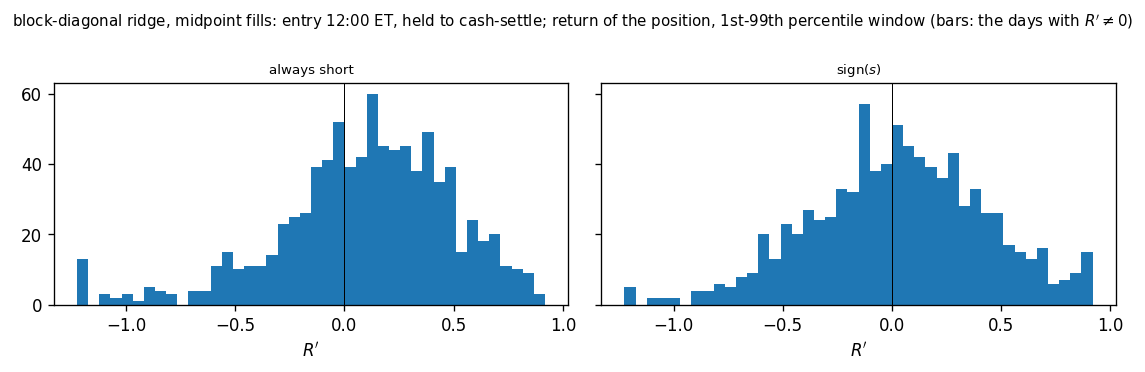
\includegraphics[width=0.45\textwidth]{../results/atm_straddle_intraday_holdclose/rule_by_strategy_dh/1200/rule_hists_blk2_1200.png}\par\smallskip
\small Distribution of the return of the position taken at 12:00 ET, block-diagonal ridge forecast, one panel per rule (returns inside their 1st--99th percentile window).
\end{center}
\vspace{1ex}
\noindent\small One trade a day: enter the nearest-OTM straddle at 12:00 ET, hold those strikes to the official close, and delta-hedge every 30 minutes. 866 expiration days, 2020-01-03 to 2024-04-30 (the deck's frame). Fills are at the quoted midpoint everywhere except the last column, which is the same rule at the crossed spread: entry at the touch (the ask when long, the bid when short) and cash-settle at the official close (no exit spread).
\vspace{1ex}
\noindent\small \textbf{Straddle} here means the nearest out-of-the-money call plus the nearest out-of-the-money put, same-day expiry, bought or sold as one position. One expiration day = one return; mid fill. Every $t$ here is the plain $t=\sqrt{n}\cdot\mathrm{mean}/\mathrm{std}$, with no autocorrelation correction. ``ex.\ kurt'' is the bias-corrected sample excess kurtosis (Gaussian $=0$). The short-volatility rule takes no forecast, so it is one row for all models. \textbf{Two Sharpes.} Both multiply by $\sqrt{252}$ because an expiration day is the unit of time (same year-length as the paper). They are not the same object. On a \emph{single-clock} page, Sharpe$_{\mathrm{clk}}=(\mathrm{mean}/\mathrm{std})\times\sqrt{252}$ of that clock's series: one remaining-session short per expiration day (enter at this clock, hold those strikes to the close, delta-hedge every 30 minutes). It answers ``if I only entered at this clock, what is my annual Sharpe?'' It is \emph{not} the book's Sharpe$_{\mathrm{ann}}$. On the \emph{pooled} page, Sharpe$_{\mathrm{ann}}=(\mathrm{mean}/\mathrm{std})\times\sqrt{252}$ of $R^{day}_d=\sum_t R'_{d,t}$, the sum of the day's thirteen overlapping remaining-session books. That reserved name is the book's daily P\&L after pooling the session. The thirteen books overlap; they are not thirteen successive holds. Sharpe$^{\times}$ is the same convention at the crossed spread. Every other column is daily. $n_{\mathrm{buy}}$ is the number of expiration days with position $>0$ (always-short is 0; on the pooled page it is days the sum of the thirteen positions is positive); \%buy is $100\cdot n_{\mathrm{buy}}/n$, the notebook's column. The other column this table adds to the deck's is Sharpe$^{\times}_{\mathrm{ann}}$, the same rule's annualized Sharpe at the \emph{crossed spread} instead of the midpoint; every other column is the deck's.

\smallskip
\noindent\small Forecasts: baseline (HAR + calendar OLS); block-diagonal ridge (HAR block and exogenous block, separate penalties) on the design carrying the FOMC calendar block, and the same ridge on the earlier design without those columns, as a diagnostic row; LightGBM and XGBoost on the all-features design; lasso on the same design, causally tuned vs.\ fixed $\alpha=10^{-4}$; elastic net (causally tuned). $\dagger$ marks a column still fitted on the earlier design panel; a run of those four on the panel of record is pending. The signal is $s_t=\widehat{RV}_t-\mathrm{IV}^{2}_{\mathrm{hr}}h_t w_t$: the forecast against the implied variance of the same window. $w_t$ is the expanding mean of each prior day's remaining-session share of realized variance, $\mathrm{RV}_t/\sum_{s\ge t}\mathrm{RV}_s$ (in-fit panel history back to 2001), not the ratio of trailing clock-means. On the bars whose vendor implied volatility is a censored solver node the deck's treatment is used here too --- the volatility that reproduces the straddle midpoint, recovered by bisection over the remaining $h_t$ hours --- so every bar carries a signal and no bar sits flat. At the 09:35 entry the forecast is the one issued at 09:30 for the 09:30--10:00 bar, $w_t$ is that bar's share, and $h_t$ is the chain's hours to the close.
\end{document}
